% THIS IS SIGPROC-SP.TEX - VERSION 3.1
% WORKS WITH V3.2SP OF ACM_PROC_ARTICLE-SP.CLS
% APRIL 2009
%
% It is an example file showing how to use the 'acm_proc_article-sp.cls' V3.2SP
% LaTeX2e document class file for Conference Proceedings submissions.
% ----------------------------------------------------------------------------------------------------------------
% This .tex file (and associated .cls V3.2SP) *DOES NOT* produce:
%       1) The Permission Statement
%       2) The Conference (location) Info information
%       3) The Copyright Line with ACM data
%       4) Page numbering
% ---------------------------------------------------------------------------------------------------------------
% It is an example which *does* use the .bib file (from which the .bbl file
% is produced).
%TODO:
% REMEMBER HOWEVER: After having produced the .bbl file,
% and prior to final submission,
% you need to 'insert'  your .bbl file into your source .tex file so as to provide
% ONE 'self-contained' source file.
%
% Questions regarding SIGS should be sent to
% Adrienne Griscti ---> griscti@acm.org
%
% Questions/suggestions regarding the guidelines, .tex and .cls files, etc. to
% Gerald Murray ---> murray@hq.acm.org
%
% For tracking purposes - this is V3.1SP - APRIL 2009

\documentclass{acm_proc_article-sp}

\usepackage{listings}
\usepackage[textwidth=0.3\textwidth,textsize=footnotesize]{todonotes}
\newcommand{\note}[1]{\todo[inline,color=yellow,bordercolor=orange,linecolor=orange]{#1}}

\begin{document}

\title{On the Composition and Exponentiation of Stencil Kernels -- Improving Performance and Energy Consumption}
%TODO: check if we need this
%% \subtitle{[Extended Abstract]
%% \titlenote{A full version of this paper is available as
%% \textit{Author's Guide to Preparing ACM SIG Proceedings Using
%% \LaTeX$2_\epsilon$\ and BibTeX} at
%% \texttt{www.acm.org/eaddress.htm}}}


\numberofauthors{3}
\author{
% 1st. author
\alignauthor
Daniel Rubio Bonilla\\
       \affaddr{High Performance Computing Center Stuttgart (HLRS)}\\
       \affaddr{University of Stuttgart}\\
       \affaddr{Stuttgart, Germany}\\
       \email{rubio@hlrs.de}
% 2nd. author
\alignauthor
Manuel Carro Li{\~n}ares\\
       \affaddr{IMDEA Software}\\
       \affaddr{Madrid, Spain}\\
       \email{manuel.carro@imdea.org}
% 3rd. author
\alignauthor
Colin W. Glass\\
       \affaddr{High Performance Computing Center Stuttgart (HLRS)}\\
       \affaddr{University of Stuttgart}\\
       \affaddr{Stuttgart, Germany}\\
       \email{glass@hlrs.de}
}

\date{30 August 2015}

\maketitle

%%%%%%%%%%%%%%%%%%%%%%%%%%%%%%%%%%%%%%%%%%%%%%%%%%%%%%%
%%%%%%%%%%%%%%%%%%%%%%%%%%%%%%%%%%%%%%%%%%%%%%%%%%%%%%%
%%%%%%%%%%%%%%%%%%%%%%%%%%%%%%%%%%%%%%%%%%%%%%%%%%%%%%%

\begin{abstract}
\note{TODO: a native speaker should check the whole document.}
Many High-Performance Computing (HPC) programs perform array or n-dimensional matrix computations that involve a class of kernels known as stencils that characterize for updating every element according to some fixed pattern. Stencils are commonly used in solving partial differential equations (used in scientific problems), image processing and geometric modeling.

In this paper we present a method to combine stencil kernel(s) that are executed iteratively, or subsequently, into one kernel to reduce the number of iterations or number of stencil kernels applied. Our empirical results show that in most cases and for different hardware families, ranging from embedded systems to HPC this strategy improves performance and reduces energy consumption.
\end{abstract}

\note{TODO: check for the right categories}
% A category with the (minimum) three required fields
\category{H.4}{Information Systems Applications}{Miscellaneous}
%A category including the fourth, optional field follows...
\category{D.2.8}{Software Engineering}{Metrics}[complexity measures, performance measures]

\terms{Theory}

\keywords{HPC, stencil, optimization, energy, performance, algorithms}

\section{Introduction}
Stencil codes are a class of iterative kernels which update array elements according to some fixed pattern, called stencil\cite{roth:hpf}. In numerical analysis a stencil is a geometric arrangement of a nodal group relative to the point of interest used to offer a numerical solution of partial differential equations or apply filters to image among other uses. For this reason they are often found in computer scientific and engineering simulation code, \textit{e.g.} for computational fluid dynamics.

Stencil codes perform a sequence of repetitive steps through a given array or matrix that generally is a 2- or 3-dimensional regular grid\cite{dietmar:cs}. In each step the stencil code updates all array elements, called cells, with a new value that is computed using for the calculation the neighbor array elements in a fixed pattern\cite{leopold:tbcm}. In most cases boundary values are left unchanged, but in some cases those need to be adjusted during the course of the computation as well. Since the stencil computation is the same for each element, the pattern of data accesses is repeated\cite{chancaoguo:hpcpi}; computationally a stencil represent a pattern of accessing to memory, as for calculating the next step value of an element in a grid, it will need its current value and the current value of a set of neighbors defined by its distance to them.

It is important to increase the performance and reduce the energy consumption of the stencil kernels, not only because they are very relevant and commonly used in image processing, and scientific and engineering codes, but also because they often result in a high percentage of the total computational resources of these applications.

In this paper we describe a new technique that is based on mathematical understanding and manipulation of the stencil mathematical expressions, that as shown by empirical results it often leads to shorter execution times and lower energy usage. In Section~\ref{maths} we describe the process of stencil exponentiation and composition then in Section~\ref{usecase} we present a use case and apply this technique to 1-, 2- and 3-dimensional stencils and analyze their theoretical computational cost. In Section~\ref{performance} the results of the benchmarks are exposed and analyzed. And finally, in Section~\ref{conclusions} the usability and improvements on this technique are discussed.


\section{Related Work}
\note{extend and detailed it more?}
Due to the high relevance of stencil computations many approaches have been develop to accelerate and improve the performance of these algorithms. Most approaches are based on improving the data locality~\cite{gysi:modesto}, such as blocking data in cache so that it can be reused~\cite{gw:eftb},
or and changing the computational order to allow vectorization. Both of these approaches are commonly used like, for example, by the PLUTO tool, an automatic parallelization tool based on the polyhedral model, which tunes the code to exploit data locality and vectorization, introduce memory management optimizations and perform automatic parallelization~\cite{bondhugula:pluto} amont others.

Up to now the most common ways of optimizing stencil codes played with how the code is executed. The approach described in this work is manipulating the mathematical formulation of the stencil. This implies that the technique here described can be also complemented with the common optimization strategies for stencils.

\note{Move pluto benchmarks to results?}
To analyze the feasibility of combining both approaches we took a 1-D stencil given as part of the PLUTO examples and we composed it. Then to both approaches we used PLUTO to optimize data locality, vectorize the code and parallelize it, resulting in four different codes; the original code, the composed code, the original code after PLUTO and the composed code after PLUTO. Figures~\ref{pic:pluto-performance} and~\ref{pic:pluto-energy} show the execution time and energy consumed to execute the different versions of the stencil on different hardware. 

\note{correct pictures}
\begin{figure}[ht!]
  \centering
  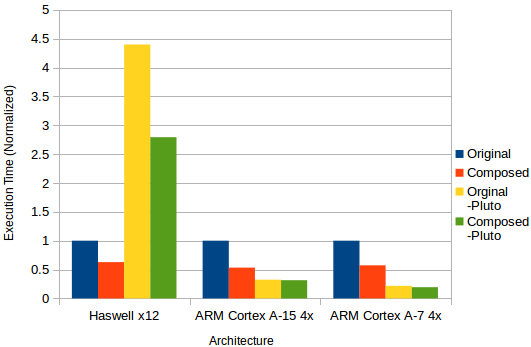
\includegraphics[scale=0.6]{results/pluto-benchmark-performance}
  \caption{Pluto and Stencil Composition - Performance (Normalized)}
  \label{pic:pluto-performance}
\end{figure}

\begin{figure}[ht!]
  \centering
  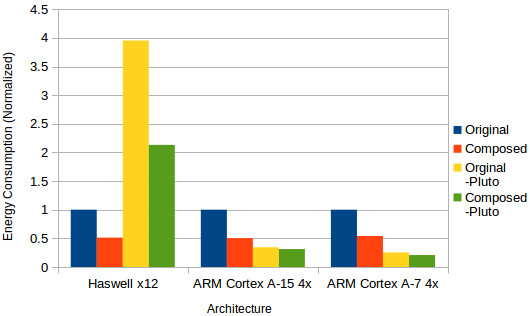
\includegraphics[scale=0.6]{results/pluto-benchmark-energy}
  \caption{Pluto and Stencil Composition - Energy (Normalized)}
  \label{pic:pluto-energy}
\end{figure}

\note{Maybe remove this note?}
We used the 1-D stencil example given by PLUTO as we failed to generate correct code from our more complex stencil codes that were used for the other benchmarks.


\section{Stencil Composition}
\label{maths}
\note{TODO: improve the mathematical formalization of the problem and solution}
Function Composition, in computer science, is a way to combine simple functions\footnote{Real-valued functions over a subset of the real-line that are measurable} to build more complex functions, where the result of each function is passed as the argument of the next function, and the result of the last one is the result of the whole\cite{lamport:cs}.
Often developers directly apply the result of one function as the argument(s) of another function a feature that is allowed by most programming languages because the ability to easily compose functions encourages factoring functions for maintainability and code reuse. In the next C code \texttt{z1} and \texttt{z2} are equivalent.
\begin{lstlisting}
y  = g(x);
z1 = f(y);

z2 = f(g(x));
\end{lstlisting}

In functional languages (Haskell is used for this example), the function composition can be expressed as:
\begin{lstlisting}
z = f . g
\end{lstlisting}
using the built-in operator (.), which can be read as \textit{f after g} or \textit{g composed with f}. Where one of the possible definitions of the (.) operator is:
\begin{lstlisting}
(.) :: (b -> c) -> (a -> b) -> a -> c
f . g = \x -> f (g x)
\end{lstlisting}

In our context, a stencil code is a function that is usually applied to all the elements of a n-dimensional array, taking as parameters a fixed pattern of neighbors elements, and the result is used to update the value of the element to which it is applied. In many applications different stencil functions are applied subsequently or the same stencil function is applied iteratively.
Composing the stencils functions result on a new equivalent function with a different (broader) geometrical pattern over the input data, but reducing the number of iterations over the data array.


\subsection{Composition of Different Stencils}
Given an application that uses two different stencil functions $g()$ and $f()$ that are applied to all elements of an n-dimensional array $V[]$ with $VN$ elements so that $V'[] = g(V[])$ and $V''[] = f(V'[]) = f(g(V[]))$ then we can define the function $z()$ so that $V''[] = z(V[])$.

Being $a_i[]$ the set of elements of $V[]$ that are the input parameters for $g()$ to obtain the value of an specific element of $V'[]$, $V'[i]$, so that $V'[i] = g(a_i[])$ and being $b_j[]$ the set of elements of $V'[]$ that are the input parameters for $f()$ to obtain the value of an specific element of $V''[]$, $V''[j]$, so that $V''[j] = f(b_j[])$. Then we can replace each element of $b_j[]$ by the pair of function $f()$ and input parameters of the array $V[]$, $a_{ij}[]$ that give each element of $b_j[]$. Replacing them in $g()$ allows us to obtain $z()$.

In summary, the composed stencil function $z()$ is obtained by replacing the parameters of $g()$ with their dependence on function $f()$ on the original elements of the array. Lets see if with an example. If\\
$V'[i] = f(V[i-1], V[i], V[i+1]) = V[i-1] + V[i+1] - V[i]$ and \\
$V''[i] = g(V'[i-1], V'[i], V'[i+1]) = V'[i] - V'[i-1] - V'[i+1]$
then each element $V'[i-1]$, $V'[i]$ and $V'[i+1]$ can be replaced with their equivalents on depending on $f()$:
$g(V'[i-1], V'[i], V'[i+1]) = V[i-1] + V[i+1] - V[i] - V[i-2] - V[i] + V[i-1]  -V[i] - V[i+2] + V[i+1] = z(V[i-2], V[i-1], V[i], V[i+1], V[i+2])$




%%%%%%%%%%%%%%%%%%%%%%%%%%%%%%%%%%%%%%%%%%%%%%%%%%%%%%%
%%%%%%%%%%%%%%%%%%%%%%%%%%%%%%%%%%%%%%%%%%%%%%%%%%%%%%%

%% Given an application that uses two different stencil functions $g()$ and $f()$ that are applied to all elements of an n-dimensional array $V[]$ with elements $v_{d1,d2,..., dn}$ where $d1 \in 0..D1\_Size$, $d2 \in 0..D2\_Size$, ..., $dn \in 0..Dn\_Size$, $G_{x1,x2,...,xn}$ the group of elements that are input parameters of the stencil $g$ for the element $v_{x1,x2,...,xn}$ and $F_{x1,x2,...,xn}$ the group of elements that are input parameters of the stencil $f$ for the element $v_{x1,x2,...,xn}$, then if $z$ is defined as $g$ composed with $f$, 

%% In summary, the resulting stencil function $z$ will have as input parameters the set of elements of
%% $z = f . g$



%% \subsubsection{1-D Stencil Composition example}
%% Given a 1-dimensional array $V = [v_0 ... v_n] : n \in \mathbb{N}$, that $V' = [v'_0 ... v'_n] : i \in [0,n]: v'_i = g(v_{i-1}, v_i, v_{i+1})$, and $V'' = [v''_0 ... v''_n] : i \in [0,n]: v''_i = f(v'_{i-1}, v'_i, v'_{i+1})$ then $z$ that is $g$ composed with $f$, can be applied to all elements of $V$ resulting in $V''$:

%% $V'' = [v''_0 ... v''_n] : i \in [0,n]: v''_i =$ \\
%% $f(g(v_{i-2}, v_{i-1}, v_{i}), g(v_{i-1}, v_i, v_{i+1}), g(v_{i}, v_{i+1}, v_{i+2})) =$ \\
%% $z(v_{i-2}, v_{i-1}, v_i, v_{i+1}, v_{i+2})$

\subsection{Stencil Exponentiation}
Stencil Exponentiation is a particular case of stencil composition. Using the same approach, instead of composing two different functions, we compose the same function with itself. Given the stencil function $f$ that is applied iteratively over a particular data-set, it can be composed with itself, $f^2 = f . f$, resulting in a powered stencil function that has to be applied half of the times to obtain the same result.


\section{Stencil Composition Aplied to a Use Case}
\label{usecase}
The heat equation is a parabolic partial differential equation that describes the variation in temperature in a given region over time.
\begin{equation}
  \frac{\partial u}{\partial t}-\alpha\nabla^{2}u=0
  \label{eqn:heo}
\end{equation}
where $u$ is the temperature at a certain location, $t$ is the time variable, $\alpha$ is the thermal diffusivity (a positive constant of the material) and $\nabla$ denotes the Laplace operator\cite{cn:he}.

In this work we examine the performance of the explicit heat equation --in 1-, 2- and 3-dimensions--, before and after composing it with itself (\textit{i.e.} exponentiation of the computational stencil kernel). First we will demonstrate on how to compose the equation from the algorithmic point of view, then we will analyze the computational cost of the different versions and to finalize, in Section~\ref{performance} we will show the performance and energy benchmarks on different platforms (different HPC and embedded systems).

\subsection{Generation of the composed stencil code}
The discretization of the partial differential equation~\eqref{eqn:heo} for the different n-dimensional cases that we are going to analyze is done using the Finite Difference Method (FDM), which is one of the dominant approaches to obtain numerical solutions of partial differential equations\cite{grossman:ntpde}.

For this work We considered a \textit{phantom halo} with null values around the original data-set so that the same stencil function, conventional or composed, can be applied to all the elements of original data. This way the need to create special functions for the borders and corners of the n-dimensional matrices is avoided. The concrete details of the tests are exposed later in Section~\ref{performance}.


\subsubsection{1-D Composed Stencil}
\label{Generation1D}
The discretization of the equation~\eqref{eqn:heo} for a 1-Dimensional space can be expressed as
\begin{equation}
  \begin{split}
    b[i] = a[i] + D(a[i-1] - 2a[i] + a[i+1])
    %b[i] = a[i] + D * (a[i-1] - 2*a[i] + a[i+1])
  \end{split}
  \label{eqn:hed-1d}
\end{equation}
where $D$ is the thermal diffusivity, the vector $a[]$ holds the input data and the vector $b[]$ stores the result of the application of the stencil over the elements of $a[]$. Figure~\ref{pic:1d-s01} shows the accessed data-pattern for reading (black and red dots in the $a[]$ data array) and data written (red dot in the $b[]$ data array). It is not possible to read and write directly to the array $a[]$ because the computation $a[i+1]$ depends on the data in $a[i]$ before applying the stencil computation to $a[i]$ (\textit{i.e.} there is a Read After Write --RAW-- data dependency between all elements of $a[]$).
\begin{figure}[ht!]
  \centering
  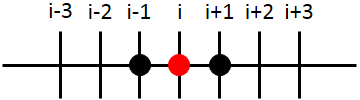
\includegraphics[scale=0.5]{pics/stencil_grid/1d-s01}
  \caption{1D Stencil -- read from black and red dot positions, write to red dot position}
  \label{pic:1d-s01}
\end{figure}

If we define the function $s()$ as the function that applied to $a[]$ returns $b[]$ so that $b[]=s(a[])$, then it can also define $t$ as $s^2()$ so that
\begin{equation}
  \begin{split}
    c[] = t(a[]) = s^2(a[]) = s(s(a[])) = s(b[])
    %$c[] = t(a[]) = s^2(a[]) = s(s(a[])) = s(b[])$
  \end{split}
  \label{eqn:hed-1dcomp}
\end{equation}
\textit{i.e.} $c[]$ is the array that stores the results of applying twice the original stencil kernel to all the elements of the original data-set $a[]$. To generate the function $t$ and knowing that it is equivalent to $s(b[])$ as seen in equation~\eqref{eqn:hed-1dcomp}, then we can express it for a particular element of $a[]$ as
\begin{equation}
  \begin{split}
    t(a[i]) = s(b[i]) = b[i] + D(b[i-1] - 2b[i] + b[i+1])
  \end{split}
  \label{eqn:hed-1dcomp2}
\end{equation}
and knowing that 
\begin{equation}
  \begin{split}
    b[i-1] = a[i-1] + D(a[i-2] - 2a[i-1] + a[i])
    %&b[i] = a[i] + D(a[i-1] - 2a[i] + a[i+1])\\
    %&b[i+1] = a[i+1] + D(a[i] - 2a[i+1] + a[i+2])
  \end{split}
  \label{eqn:hed-1dp}
\end{equation}
\begin{equation}
  \begin{split}
    %&b[i-1] = a[i-1] + D(a[i-2] - 2a[i-1] + a[i])\\
    %&b[i] = a[i] + D(a[i-1] - 2a[i] + a[i+1])\\
    b[i+1] = a[i+1] + D(a[i] - 2a[i+1] + a[i+2])
  \end{split}
  \label{eqn:hed-1dp}
\end{equation}
with their relative data access pattern depicted in Figure~\ref{pic:1d-s01all} for $b[i-1]$ and for $b[i+1]$,
\begin{figure}[ht!]
  \centering
  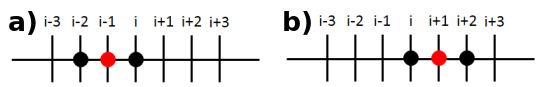
\includegraphics[scale=0.6]{pics/stencil_grid/1d-s01_all}
  \caption{1D Stencil -- relative data access pattern for $b[i-1]$ and $b[i+1]$}
  \label{pic:1d-s01all}
\end{figure}

%% \begin{figure}[ht!]
%%   \centering
%%   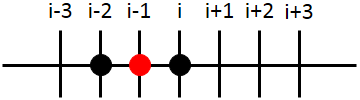
\includegraphics[scale=0.5]{pics/stencil_grid/1d-s01a}
%%   \caption{1D Stencil -- relative data access pattern for $b[i-1]$}
%%   \label{pic:1d-s01a}
%% \end{figure}

%% \begin{figure}[ht!]
%%   \centering
%%   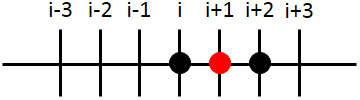
\includegraphics[scale=0.5]{pics/stencil_grid/1d-s01b}
%%   \caption{1D Stencil -- relative data access pattern for $b[i+1]$}
%%   \label{pic:1d-s01b}
%% \end{figure}
we can apply the substitutions of $b[i-1]$, $b[i]$ and $b[i+1]$ in equation~\eqref{eqn:hed-1dcomp2} resulting in
\begin{equation}
  %\tag{d}
  \begin{split}
    t(a[i]) &= c[i]\\
    c[i] &= a[i] + D(a[i-1] - 2a[i] + a[i+1])\\
    &+ D(a[i-1] + D(a[i-2] - 2a[i-1] + a[i])\\
    &- 2(a[i] + D(a[i-1] - 2a[i] + a[i+1]))\\
    &+ a[i+1] + D(a[i] - 2a[i+1] + a[i+2]))
  \end{split}
  \label{eqn:hed-1dcomp2b}
\end{equation}
After the direct substitution of the terms, eliminating the intermediary step $b[]$, the equation~\eqref{eqn:hed-1dcomp2b} can be simplified to the equation~\eqref{eqn:hed-1dcomp2c}.
\begin{equation}
  %\tag{d}
  \begin{split}
    c[i] &= D^2(a[i-2]+a[i+2])\\
       &+ (2D-4D^2)(a[i-1]+a[i+1])\\ 
       &+ (1-4D+6D^2)a[i];
  \end{split}
  \label{eqn:hed-1dcomp2c}
\end{equation}
The new data access pattern of equation~\eqref{eqn:hed-1dcomp2c} is graphically represented in Figure~\ref{pic:1d-s02}. It can be observed that the geometrical pattern of input data has broadened to include all the elements of the access pattern needed to compute $b[i-1]$, $b[i]$, $b[i+1]$. 
\begin{figure}[ht!]
  \centering
  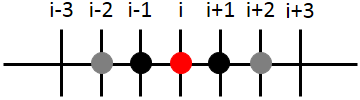
\includegraphics[scale=0.5]{pics/stencil_grid/1d-s02}
  \caption{1D Stencil -- Composed Heat Equation Stencil data access pattern}
  \label{pic:1d-s02}
\end{figure}




\subsubsection{2-D Composed Stencil}
\label{Generation2D}
The discretization of the equation~\eqref{eqn:heo} for a 2-Dimensional space can be expressed as
\begin{equation}
  %\tag{c}
  \begin{split}
    b[j,i] &= a[j,i] + D(a[j-1,i] + a[j,i-1] - 4a[j,i]\\
    &+ a[j,i+1] + a[j+1,i])
    %b[j,i] &= a[j,i] + D * (a[j-1,i] + a[j,i-1] - 4*a[j,i]\\
    %&+ a[j,i+1] + a[j+1,i])
  \end{split}
  \label{eqn:hed-2d}
\end{equation}
where $D$ is the thermal diffusivity, the vector $a[]$ holds the input data and the vector $b[]$ stores the result of the application of the stencil over the elements of $a[]$. Figure~\ref{pic:2d-s01} shows the accessed data for reading (black and red dots in the $a[]$ data array) and data written (red dot in the $b[]$ data array).

As we have seen in Section~\ref{Generation1D}, it is not possible to read and write directly to the array $a[]$ because of the algorithmic RAW data dependencies between the elements of $a[]$.
\begin{figure}[ht!]
  \centering
  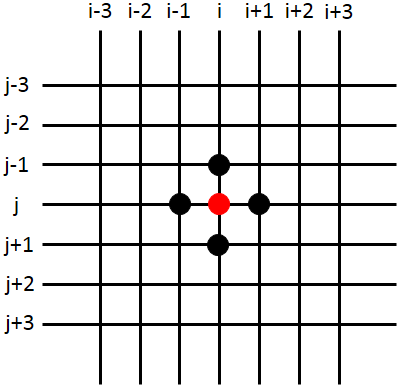
\includegraphics[scale=0.5]{pics/stencil_grid/2d-s01}
  \caption{2D Stencil -- read from black and red dot positions, write to red dot position}
  \label{pic:2d-s01}
\end{figure}

Similarly as in the 1-Dimensional case we can define the function $s()$ as the function that applied to $a[]$ returns $b[]$ so that $b[]=s(a[])$, then it can also define $t$ as $s^2()$ so that
\begin{equation}
  \begin{split}
    c[] = t(a[]) = s^2(a[]) = s(s(a[])) = s(b[])
  \end{split}
  \label{eqn:hed-2dcomp}
\end{equation}
where $c[]$ is the array that stores the results of applying twice the original stencil kernel to all the elements of the original data-set $a[]$. As previously seen, to generate the function $t$ and knowing that it is equivalent to $s(b[])$ as seen in equation~\eqref{eqn:hed-2dcomp}, then we can express it for a specific element of $a[]$ as
\begin{equation}
  %\tag{d}
  \begin{split}
    t(a[j,i]) &= s(b[j,i]) = b[j,i] + D(b[j-1,i]\\
    &+ b[j,i-1] - 4b[j,i] + b[j,i+1] + b[j+1,i])
  \end{split}
  \label{eqn:hed-2dcomp2}
\end{equation}
and knowing that 
\begin{equation}
  \begin{split}
    b[j-1,i] &= a[j-1,i] + D(a[j-2,i] + a[j-1,i-1]\\
    &- 4a[j-1,i] + a[j-1,i+1] + a[j,i])\\
    % a[j-1,i] + D(a[j-2,i] + a[j-1,i-1]- 4a[j-1,i] + a[j-1,i+1] + a[j,i])
  \end{split}
  \label{eqn:hed-2alla}
\end{equation}
\begin{equation}
  \begin{split}
    b[j,i-1] &= a[j,i-1] + D(a[j-1,i-1] + a[j,i-2]\\
    &- 4a[j,i-1] + a[j,i] + a[j+1,i-1])\\
    % a[j,i-1] + D(a[j-1,i-1] + a[j,i-2]- 4a[j,i-1] + a[j,i] + a[j+1,i-1])
  \end{split}
  \label{eqn:hed-2allb}
\end{equation}
\begin{equation}
  \begin{split}
    b[j,i+1] &= a[j,i+1] + D(a[j-1,i+1] + a[j,i]\\
    &- 4a[j,i+1] + a[j,i+2] + a[j+1,i+1])\\
    %a[j,i+1] + D(a[j-1,i+1] + a[j,i]- 4a[j,i+1] + a[j,i+2] + a[j+1,i+1])
  \end{split}
  \label{eqn:hed-2alld}
\end{equation}
\begin{equation}
  \begin{split}
    b[j+1,i] &= a[j+1,i] + D(a[j,i] + a[j+1,i-1]\\
    &- 4a[j+1,i] + a[j+1,i+1] + a[j+2,i])
    % a[j+1,i] + D(a[j,i] + a[j+1,i-1]- 4a[j+1,i] + a[j+1,i+1] + a[j+2,i])
  \end{split}
  \label{eqn:hed-2alle}
\end{equation}
with their relative data access pattern depicted in Figure~\ref{pic:2d-s01}
\begin{figure}[ht!]
  \centering
  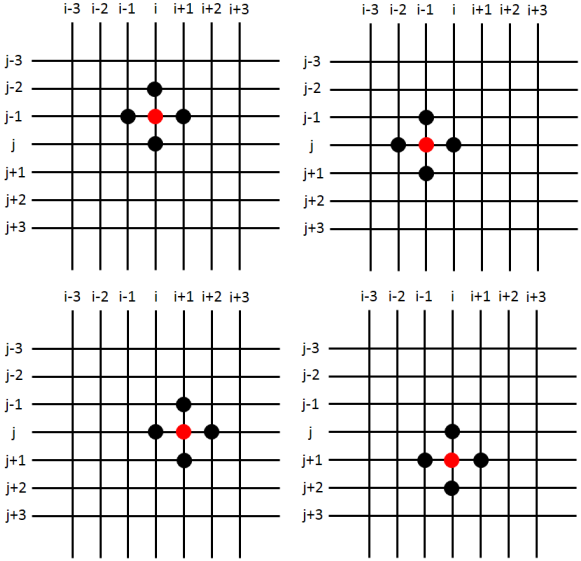
\includegraphics[scale=0.5]{pics/stencil_grid/2d-s01_all}
  \caption{2D Stencil -- read from black and red dot positions, write to red dot position}
  \label{pic:2d-s01}
\end{figure}
the substitutions (equations~\eqref{eqn:hed-2d}, \eqref{eqn:hed-2alla}, \eqref{eqn:hed-2allb}, \eqref{eqn:hed-2alld} and~\eqref{eqn:hed-2alle}) can be directly applied to equation~\eqref{eqn:hed-2dcomp2} resulting in
\begin{equation}
  %\tag{d}
  \begin{split}
    t(a[j,i]) &= c[j,i]\\
    c[j,i] &= a[j,i] + D(a[j-1,i] + a[j,i-1] - 4a[j,i]\\
    &+ a[j,i+1] + a[j+1,i]) + D(a[j-1,i]\\
    &+ D(a[j-2,i] + a[j-1,i-1]- 4a[j-1,i]\\
    &+ a[j-1,i+1] + a[j,i]) + a[j,i-1]\\
    &+ D(a[j-1,i-1] + a[j,i-2]- 4a[j,i-1]\\
    &+ a[j,i] + a[j+1,i-1]) - 4(a[j,i]\\
    &+ D(a[j-1,i] + a[j,i-1] - 4a[j,i]\\
    &+ a[j,i+1] + a[j+1,i])) + a[j,i+1]\\
    &+ D(a[j-1,i+1] + a[j,i]- 4a[j,i+1]\\
    &+ a[j,i+2] + a[j+1,i+1]) + a[j+1,i]\\
    &+ D(a[j,i] + a[j+1,i-1]- 4a[j+1,i]\\
    &+ a[j+1,i+1] + a[j+2,i]))
  \end{split}
  \label{eqn:hed-2dcomp}
\end{equation}
The resulting equation after the direct substitution of the terms, eliminating the intermediary step $b[]$, the equation~\eqref{eqn:hed-2dcomp} can be simplified to the equation~\eqref{eqn:hed-2dcomps}.
\begin{equation}
  \begin{split}
    c[j,i] &= D^2(a[j-2,i] + a[j,i-2] + a[j,i+2]\\
    &+ a[j+2,i]) + (2D^2)(a[j-1,i-1]\\
    &+ a[j-1,i+1]+a[j+1,i-1]+a[j+1,i+1])\\
    &+ (2D-8D^2)(a[j-1,i]+a[j,i-1]+a[j,i+1]\\
    &+a[j+1,i]) + (1-8D+20D^2)(a[j,i])
  \end{split}
  \label{eqn:hed-2dcomps}
\end{equation}
The new data access geometrical pattern of equation~\eqref{eqn:hed-2dcomps} is graphically represented in Figure~\ref{pic:2d-s02}.
\begin{figure}[ht!]
  \centering
  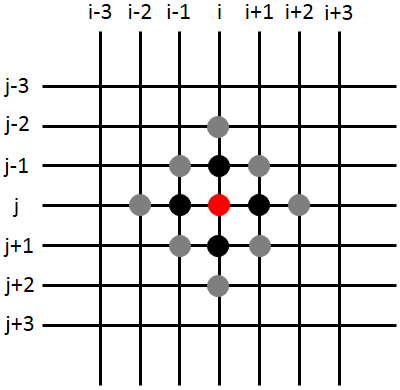
\includegraphics[scale=0.5]{pics/stencil_grid/2d-s02}
  \caption{2D Stencil -- Composed Heat Equation Stencil data access pattern}
  \label{pic:2d-s02}
\end{figure}



\subsubsection{3-D Composed Stencil}
The discretization of the equation~\eqref{eqn:heo} for a 3-Dimensional space can be expressed as
\begin{equation}
  %\tag{d}
  \begin{split}
    b[k,j,i] &= a[k,j,i] + D(a[k-1,j,i]\\
    &+ a[k,j-1,i] + a[k,j,i-1] - 6a[k,j,i]\\
    &+ a[k,j,i+1] + a[k,j+1,i] + a[k+1,j,i])
    %b[k,j,i] &= a[k,j,i] + D * (a[k-1,j,i]\\
    %&+ a[k,j-1,i] + a[k,j,i-1] - 6*a[k,j,i]\\
    %&+ a[k,j,i+1] + a[k,j+1,i] + a[k+1,j,i])
  \end{split}
  \label{eqn:hed-3d}
\end{equation}
where $D$ is the thermal diffusivity, the vector $a[]$ holds the input data and the vector $b[]$ stores the result of the application of the stencil over the elements of $a[]$. Figure~\ref{pic:3d-s01} shows the accessed data for reading (black and red dots in the $a[]$ data array) and data written (red dot in the $b[]$ data array).
In this case, similarly to the 1-D and 2-D versions of this problem (Sections~\ref{Generation1D} and~\ref{Generation2D}), it is not possible to read and write directly to the array $a[]$ because of the algorithmic RAW data dependencies between the elements of $a[]$.
\begin{figure}[ht!]
  \centering
  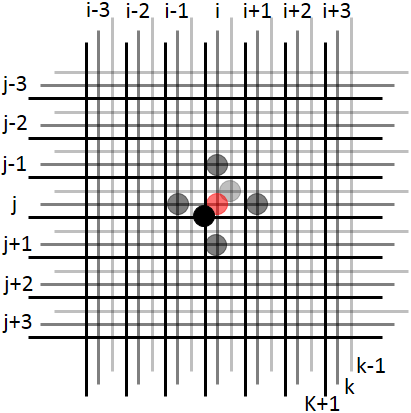
\includegraphics[scale=0.5]{pics/stencil_grid/3d-s01}
  \caption{3D Stencil -- read from black and red dot positions, write to red dot position}
  \label{pic:3d-s01}
\end{figure}

As in the previous 1-D and 2-D cases, we can define the function $s()$ as the function that applied to $a[]$ returns $b[]$ so that $b[]=s(a[])$, then it can also define $t$ as $s^2()$ so that
\begin{equation}
  \begin{split}
    c[] = t(a[]) = s^2(a[]) = s(s(a[])) = s(b[])
  \end{split}
  \label{eqn:hed-3dcomp}
\end{equation}
where $c[]$ is the array that stores the results of applying twice the original stencil kernel to all the elements of the original data-set $a[]$. As previously seen, to generate the function $t$ and knowing that it is equivalent to $s(b[])$ as seen in equation~\eqref{eqn:hed-3dcomp}, then we can express it for a specific element of $a[]$ as
\begin{equation}
  %\tag{d}
  \begin{split}
    t(a[k,j,i]) &= s(b[k,j,i]) = b[k,j,i] + D(b[k-1,j,i]\\
    &+ b[k,j-1,i] + b[k,j,i-1]\\
    &- 6b[k,j,i] + b[k,j,i+1]\\
    &+ b[k,j+1,i] + b[k+1,j,i])
  \end{split}
  \label{eqn:hed-3dcomp2}
\end{equation}
As shown in the previous sections, if the specific elements of $b[]$ that appear in the equation~\eqref{eqn:hed-3dcomp2} are replaced by their equivalents expressed as just depending on elements of $a[]$ so that all the elements of $b[]$ disappear from the equation we obtain, already simplified the equation\eqref{eqn:hed-3dcomps}.
\begin{equation}
  \begin{split}
c[k,j,i] &= (2D-6D^2)(a[k,j-1,i] + a[k,j,i-1]\\
&+ a[k,j,i+1] + a[k,j+1,i] + a[k-1,j,i]\\
&+ a[k+1,j,i]) + (2D^2)(a[k,j-1,i-1]\\
&+ a[k,j-1,i+1] + a[k-1,j-1,i]\\
&+ a[k+1,j-1,i] + a[k,j+1,i-1]\\
&+ a[k-1,j,i-1] + a[k+1,j,i-1]\\
&+ a[k,j+1,i+1] + a[k-1,j,i+1]\\
&+ a[k+1,j,i+1] + a[k-1,j+1,i]\\
&+ a[k+1,j+1,i]) + (D^2)(a[k,j-2,i]\\
&+ a[k,j,i-2] + a[k,j,i+2] + a[k,j+2,i]\\
&+ a[k-2,j,i] + a[k+2,j,i])\\
&+ (1-12D+42D^2)a[k,j,i]
  \end{split}
  \label{eqn:hed-3dcomps}
\end{equation}
In this case the data access geometrical pattern has also grown to include all the necessary \textit{points} from $a[]$ to compute at once an element of $c[]$ without the need of an intermediary grid $b[]$.

%%%%%%%%%%%%%%%%%%%%%%%%%%%%%%%%%%%%%%%%%%%%%%%%%%%%%%%
%%%%%%%%%%%%%%%%%%%%%%%%%%%%%%%%%%%%%%%%%%%%%%%%%%%%%%%
%%%%%%%%%%%%%%%%%%%%%%%%%%%%%%%%%%%%%%%%%%%%%%%%%%%%%%%


\subsection{Computational Analysis}
\label{analysis}
In this section we will analyze the number of arithmetic and memory operations needed by each version of the stencil kernels. These figures can be indicative of the benefits or detriments caused by the stencil composition, although to really answer the question on how it affects execution time and energy used, the only possibility is to execute representative application and measure it. The reason is that it is almost impossible to predict detailed behaviors on modern CPUs due to the different optimization strategies that these currently implement, such as complex memory hierarchies (\textit{i.e.} different cache levels with some levels shared across different cores), data pre-fetching, multiple execution pipelines, etc. As stencil computations are very data intensive, to determine the impact from the memory subsystem, two implementations of every formulation were developed, one with single precision and another with double precision floating point data types. Double precision uses twice the memory for each data element, 8 bytes, while single precision uses 4 bytes. The cost of computing the same operation in single or double precision might be similar, or not, depending on the hardware implementation.

\note{TODO: make tables look nicer}

\subsubsection{1-D Computational Analysis}
An equivalent formulation of equation~\eqref{eqn:hed-1d} is given in equation~\eqref{eqn:1ds}. This formulation is characterized for offering a better performance, even when it performs and extra arithmetic operation, because the number of memory operations is reduced, which is the main bottleneck as will be seen later in Section~\ref{performance}. The computational cost of these are compared in Table~\ref{tbl:1d-s01a}.
\begin{equation}
  \begin{split}
    b[i] = (1-2D)a[i]+D(a[i-1]+a[i+1])
  \end{split}
  \label{eqn:1ds}
\end{equation}

\begin{table}[ht]
  \begin{center}
    \begin{tabular}{| l | l | l |}
      \hline
       & Eq.~\eqref{eqn:hed-1d} & Eq.~\ref{eqn:1ds} \\ \hline
      ADDs   & 3 & 2 \\ \hline
      MULs   & 1 & 2 \\ \hline
      READs  & 4 & 3 \\ \hline
      WRITEs & 1 & 1 \\ \hline
    \end{tabular}
    \caption{Computational analysis of equivalent 1-D stencil formulations}
    \label{tbl:1d-s01a}
  \end{center}
\end{table}

Table~\ref{tbl:1d-s02a} compares the theoretical computational cost of executing twice equation~\eqref{eqn:1ds}, left column, with the execution of the composed stencil as formulated in equation~\eqref{eqn:hed-1dcomp2c}, right column, as these are mathematically equivalent.

\begin{table}[ht]
\begin{center}
  \begin{tabular}{| l | l | l |} \hline
     & 2x Eq.~\eqref{eqn:1ds} & Eq.~\eqref{eqn:hed-1dcomp2c} \\ \hline
    ADDs   & 4 & 4 \\ \hline
    MULs   & 4 & 3 \\ \hline
    READs  & 6 & 5 \\ \hline
    WRITEs & 2 & 1  \\ \hline
  \end{tabular}
    \caption{Computational analysis of applying twice the original 1-D stencil kernel and once the equivalent composed stencil kernel}
    \label{tbl:1d-s02a}
\end{center}
\end{table}
The composed 1-D stencil reduces some of the arithmetic and memory operations.


\subsubsection{2-D Computational Analysis}
Similarly to the 1-D version, equation~\eqref{eqn:hed-2d} can be formulated as in equation~\eqref{eqn:2ds} that is equivalent but offers better performance due to the reduction of memory operations.
\begin{equation}
  \begin{split}
    b[j,i] &= (1-4D)a[i,j] + D(a[j-1,i] + a[j,i-1]\\
    &+ a[j,i+1] + a[j+1,i]
  \end{split}
  \label{eqn:2ds}
\end{equation}

The computational cost of these are compared in Table~\ref{tbl:2d-s01a}.
\begin{table}[ht]
\begin{center}
  \begin{tabular}{| l | l | l |}
    \hline
    & Eq~\eqref{eqn:hed-2d} & Eq~\ref{eqn:2ds} \\ \hline
    ADDs   & 5 & 4 \\ \hline
    MULs   & 1 & 2 \\ \hline
    READs  & 6 & 5 \\ \hline
    WRITEs & 1 & 1 \\ \hline
  \end{tabular}
  \caption{Computational analysis of equivalent 2-D stencil formulations}
  \label{tbl:2d-s01a}
\end{center}
\end{table}


Table~\ref{tbl:2d-s02a} compares the theoretical computational cost of executing twice equation~\eqref{eqn:2ds}, left column, with the execution of the composed stencil as formulated in equation~\eqref{eqn:hed-2dcomps}, right column, as these are mathematically equivalent.
\begin{table}[ht]
\begin{center}
  \begin{tabular}{| l | l | l |} \hline
     & 2x Eq~\eqref{eqn:2ds} & Eq~\eqref{eqn:hed-2dcomps} \\ \hline
    ADDs   & 8 & 12 \\ \hline
    MULs   & 4 & 4 \\ \hline
    READs  & 10 & 13 \\ \hline
    WRITEs & 2 & 1  \\ \hline
  \end{tabular}
    \caption{Computational analysis of applying twice the original 2-D stencil kernel and once the equivalent composed stencil kernel}
    \label{tbl:2d-s02a}
\end{center}
\end{table}
Arithmetic and memory read operations have slightly increased, but write to memory operations remain lower in the composed stencil.


\subsubsection{3-D Computational Analysis}
As with the previous versions, equation~\eqref{eqn:hed-3d} can be formulated as in equation~\eqref{eqn:3ds} that is equivalent but offers better performance due to the reduction of memory operations. The computational cost of these are compared in Table~\ref{tbl:3d-s01a}.
\begin{equation}
  \begin{split}
    b[k,j,i] &= (1-6D)a[k,j,i] + D(a[k-1,j,i]\\
    &+ a[k,j-1,i] + a[k,j,i-1] + a[k,j,i+1]\\
    &+ a[k,j+1,i] + a[k+1,j,i])
  \end{split}
  \label{eqn:3ds}
\end{equation}


\begin{table}[ht]
\begin{center}
  \begin{tabular}{| l | l | l |}\hline
    & Eq~\eqref{eqn:hed-3d} & Eq~\ref{eqn:3ds} \\ \hline
    ADDs   & 7 & 6 \\ \hline
    MULs   & 1 & 2 \\ \hline
    READs  & 8 & 7 \\ \hline
    WRITEs & 1 & 1 \\ \hline
  \end{tabular}
    \caption{Computational analysis of equivalent 3-D stencil formulations}
    \label{tbl:3d-s01a}
\end{center}
\end{table}

Table~\ref{tbl:3d-s02a} compares the theoretical computational cost of executing twice equation~\eqref{eqn:3ds}, left column, with the execution of the composed stencil as formulated in equation~\eqref{eqn:hed-3dcomps}, right column, as these are mathematically equivalent.
\begin{table}[ht]
  \begin{center}
    \begin{tabular}{| l | l | l |} \hline
      & 2x Eq~\eqref{eqn:3ds} & Eq~\eqref{eqn:hed-3dcomps} \\ \hline
      ADDs   & 12 & 24 \\ \hline
      MULs   & 4 & 4 \\ \hline
      READs  & 14 & 25 \\ \hline
      WRITEs & 2 & 1  \\ \hline
    \end{tabular}
    \caption{Computational analysis of applying twice the original 3-D stencil kernel and once the equivalent composed stencil kernel}
    \label{tbl:3d-s02a}
  \end{center}
\end{table}

In this case it can be observed that most of the parameters got sensibly worse. ADD and memory READ operations are almost doubled, and only the WRITE to memory operation remains lower. For this reasons we might be tempted to think that, obviously, the execution time has to be worse. But as we will see in Chapter~\ref{performance} this is not always true, as it heavily depends on the hardware platform on which the code is executing.

%%%%%%%%%%%%%%%%%%%%%%%%%%%%%%%%%%%%%%%%%%%%%%%%%%%%%%%
%%%%%%%%%%%%%%%%%%%%%%%%%%%%%%%%%%%%%%%%%%%%%%%%%%%%%%%
%%%%%%%%%%%%%%%%%%%%%%%%%%%%%%%%%%%%%%%%%%%%%%%%%%%%%%%



\section{Empirical Performance Analysis}
\label{performance}
The composed stencils for 1-, 2- and 3-dimensions (equations~\eqref{eqn:hed-1dcomp2c}, \eqref{eqn:hed-2dcomps} and \eqref{eqn:hed-3dcomps} respectively) have been directly benchmarked against theire standard versions and formulated in equations~\eqref{eqn:1ds}, \eqref{eqn:2ds} and \eqref{eqn:3ds}. The equations were directly coded in C, \textit{e.g.} equation~\eqref{eqn:1ds} was implemented as:
\begin{lstlisting}
#define D 0.05f //Some value < 0.5
...
b[i]= (1.0f-2.0f*D)*a[i]+D*(a[i-1]+a[i+1]);
\end{lstlisting}
when \texttt{a[]} and \texttt{b[]} were arrays storing single precission floating point elements and
\begin{lstlisting}
#define D 0.05 //Some value < 0.5
...
b[i]= (1.0-2.0*D)*a[i]+D*(a[i-1]+a[i+1]);
\end{lstlisting}
when \texttt{a[]} and \texttt{b[]} were storing double precision elements. All tests were executed on different hardware, ranging from low-power embedded Cortex-A7 cores to bigger and \textit{power-hungry} Cortex-A15 cores to modern HPC Intel \textit{Haswell} cores, in single and multiple threads. These platforms are detailed in the next Section~\ref{hardware}.

The test applications applied the stencil a determined number of iterations $N$ ($N/2$ for the composed stencil, so that the final computation is equivalent) and used pointer-swapping double buffering to store the intermediate results between iterations. Table~\ref{tbl:problem} describes the size of the problem, the memory used --in single precision (SP) and double precision (DP)--, and the number of iterations the stencils were applied.

\begin{table}[ht]
  \begin{center}
    \begin{tabular}{| l | l | l |} \hline
                         & Odroid-XU3      & Hornet          \\ \hline
      \multicolumn{3}{|c|}{1-Dimension}                      \\ \hline
      Grid Size          & $96000000$      & $2097152000$    \\ \hline
      Bytes (SP/DP)      & (1.43/0.72) GiB & (16.0/32.0) GiB \\ \hline
      Iterations (Si/Co) & (200/100)       & (30/15)         \\ \hline
      \multicolumn{3}{|c|}{2-Dimensions}                     \\ \hline
      Grid Size          & $9600^2$        & $25600^2$        \\ \hline
      Bytes (SP/DP)      & (0.68/1.37) GiB & (5.0/10.0) GiB  \\ \hline
      Iterations (Si/Co) & (40/20)         & (60/30)          \\ \hline
      \multicolumn{3}{|c|}{3-Dimensions}                     \\ \hline
      Grid Size          & $400^3$         & $1280^3$         \\ \hline
      Bytes (SP/DP)      & (0.5/1.0) GiB   & (16.0/32.0) GiB \\ \hline
      Iterations (Si/Co) & (40/20)         & (20/10)         \\ \hline
    \end{tabular}
    \caption{Test size description for each platform}
    \label{tbl:problem}
  \end{center}
\end{table}


\subsection{Hardware}
\label{hardware}
The \textbf{Odroid-XU3} 
is a High Performance Embedded Board featuring 8 CPU cores in two 4-core cluster. The first cluster is formed by ARM Cortex A-7 cores (little cores -- configuration A, Table~\ref{tbl:hardware1}) and the second cluster is formed by ARM Cortex A-15 cores (big cores -- configuration B, Table~\ref{tbl:hardware2}).  The board contains 4 current and voltage sensors to measure the power consumption of the Cortex A-15 cores (big core cluster), the Cortex A-7 cores (little core cluster), GPU and DRAM individually. The underlying Operating System installed on this board is Ubuntu 14.04 LTS GNU/Linux.
\begin{table}[ht]
  \begin{center}
    \begin{tabular}{| l | p{6cm} |}
      \hline
      CPU & Samsung Exynos 5422 -- Configuration A\\ \hline
      Cores & 4x Cortex A-7 @ 1.4 Ghz  \\ \hline
      Cache & 0.5 MiB L2 (shared) \\ \hline
      RAM & 2GiB LPDDR3 @ 933MHz (14.9 GiB/s)  \\ \hline
    \end{tabular}
    \caption{Odroid-XU3 -- Configuration A -- Hardware description}
    \label{tbl:hardware1}
  \end{center}
\end{table}
\begin{table}[ht]
  \begin{center}
    \begin{tabular}{| l | p{6cm} |}
      \hline
      CPU & Samsung Exynos 5422  -- Configuration B\\ \hline
      Cores & 4x Cortex A-15 @ 2.0 Ghz  \\ \hline
      Cache & 2 MiB L2 (shared) \\ \hline
      RAM & 2GiB LPDDR3 @ 933MHz (14.9 GiB/s)  \\ \hline
    \end{tabular}
    \caption{Odroid-XU3 -- Configuration B -- Hardware description}
    \label{tbl:hardware2}
  \end{center}
\end{table}

The \textbf{Cray XC40}
is a massively parallel multiprocessor HPC system manufactured by Cray. It is based on x86-64 Intel Haswell Xeon processors and the Cray Aries network. Each computing node has the mechanism to measure and expose trough the file system the total power used from the start up till the moment of the request but unfortunately it does not report how the energy was used. Although the test machine (the Hornet system at HLRS) consists of 3944 compute nodes, only one was used for the tests as using more nodes would not contribute to the aim of this paper. The system is running a version of GNU/Linux customized by Cray and designed for this particular cluster. The tests in this platform were executed in single and double precision and using one or 24 cores.
\begin{table}[ht]
  \begin{center}
    \begin{tabular}{| l | p{6cm} |}
      \hline
      CPU & 2x Intel Xeon E5-2680v3 \\ \hline
      Cores & 24x Haswell Cores @ 2.5 Ghz  \\ \hline
      Cache L2 & 24x 0.25 MiB L2 (for each core + L1) \\ \hline
      Cache L3 & 2x 30 MiB LLC (one per CPU) \\ \hline
      RAM & 128GiB DDR4 @ 2100MHz (136 GiB/s)  \\ \hline
    \end{tabular}
    \caption{Hornet Node -- Hardware description}
    \label{tbl:hardware3}
  \end{center}
\end{table}
The Hardware of a Hornet node are detailed in Table~\ref{tbl:hardware3}.


\subsection{Methodology}
The compiler GCC 5.1 was used to generate the binaries for the Odroid-XU3 board with the options \texttt{-O3 -ffast-math}\footnote{\texttt{-ffast-math} allows the compiler to re-order floating point operations, which numerically might lead to not exactly the same results due to the representation limits and rounding in IEEE 754 technical standard~\cite{ieee:ieee754}.} as this combination of compilation flags offered the same or best performance as other flags, even better than adding \texttt{-mtune=native}, \texttt{-mtune=cortex-a15} or \texttt{-mtune=cortex-a7}. Other compilers such as GCC 4.9.2 and LLVM 3.6 were also tested but the performance of their binaries was always worse than GCC 5.1. For both different types of cores in this CPU, the tests were executed in single and double precision and using one or 4 cores (\textit{i.e.} using all the cores of each cluster).
This board integrates accurate current and voltage sensors on the PCB that allow to measure the energy consumption of the big cores (Cortex-A15 cluster), little cores (Cortex-A7 cluster), GPU and DRAM individually. Unfortunately there is no sensor for the whole system as some devices, such as the network NIC or the flash drive, are not reported. But the power needed by these devices is small compared to the CPU in active usage.

For the Cray XC40 the Cray Compiling Environment (CCE 8.3.14) was used as this specialized compiler generates binaries with better performance than other generic compilers available in the service nodes of this system. The tests in this platform were also executed in single and double precision and using one or 24 cores (\textit{i.e.} the total amount of cores in a node). Each node contains a sensor that measures the energy consumed by the whole node, without specifying how the energy was used, for this reason we will not be able to analyze how the composed stencil behaves from the energy point of view of the CPU or memory individually, but just the node as a whole.

%%%%%%%%%%%%%%%%%%%%%%%%%%%%%%%%%%%%%%%%%%%%%%%%%%%%%%%
%%%%%%%%%%%%%%%%%%%%%%%%%%%%%%%%%%%%%%%%%%%%%%%%%%%%%%%

\subsection{Results}
\label{results}
In the charts shown in this section (from Figures~\ref{pic:hornet-1d} to~\ref{pic:A7-3d}) the pairs of bars show the execution time and energy consumed to execute the same problem where the left blue bar represents the time in milliseconds and the right orange bar represents the energy used in joules; lower values of each bar mean better results.

The labels of the charts are composed by 3 groups of 2 characters. The first group can be \texttt{Si} for ``simple'' stencil (the conventional one) or \texttt{Co} for ``composed'' stencil, the one generated with the approach described in this paper. The second group can be \texttt{SP} for ``Single Precision'' or \texttt{DP} ``Double Precision'' floating point data types. The latest group can be \texttt{1T}, meaning that the test was running using only one thread (core), or \texttt{4T} running on 4 threads (on the Odroid-XU3 board) or \texttt{24T} running on 24 threads (on the Hornet HPC system).
\note{TODO: Improve charts\\ a) not blured\\ b) improve colors for B/W printing}
\note{TODO: Make Energy Tables nicer}

\noindent \textbf{1-D Composed Stencil Results} \\
From the computational analysis from Section~\ref{analysis} we can expect certain benefit of the composed stencil. This is confirmed in the empirical results where, in many cases, both execution time and energy used is halved when dual precision data types and multi-threading is used for all the kinds of hardware tested. 

%Figure~\ref{pic:hornet-1d}
\begin{figure}[ht!]
  \centering
  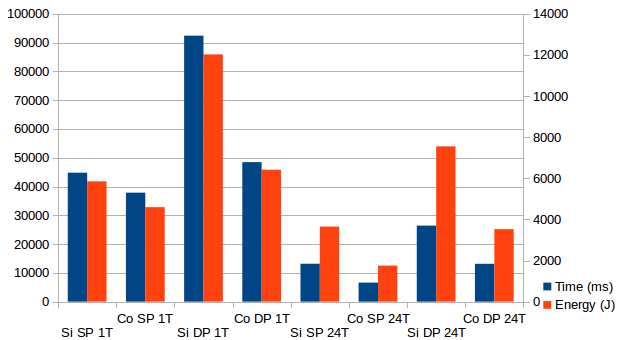
\includegraphics[scale=0.5]{results/Hornet-1D}
  \caption{Hornet 1-D Stencil benchmark}
  \label{pic:hornet-1d}
\end{figure}

%Figure~\ref{pic:A15-1d}
\begin{figure}[ht!]
  \centering
  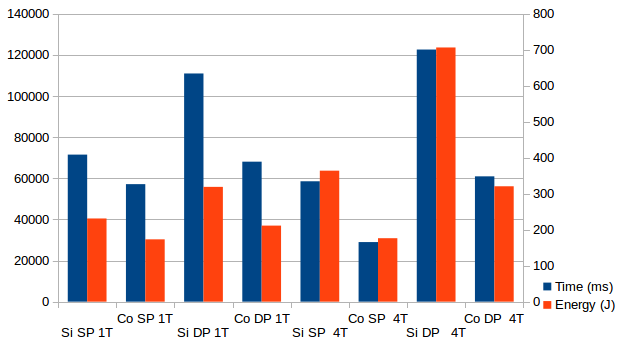
\includegraphics[scale=0.5]{results/A15-1D}
  \caption{Cortex-A15 1-D Stencil benchmark}
  \label{pic:A15-1d}
\end{figure}

Table~\ref{tbl:energy-A15-1D} shows that the not-used elements of the CPU (the Cortex-A7 cluster and the GPU) and active elements (the Cortex-A15 cluster and the memory) used energy proportional to the execution time.
\begin{table}[ht]
  \begin{center}
    \begin{tabular}{| l | l | l | l | l | l |}
      \hline
      & Total & A15 & A7 & GPU & Memory \\ \hline
      Si SP 1T & 231.42 & 206.87 & 1.97 &  8.61  & 13.96 \\ \hline
      Co SP 1T & 173.29 & 157.26 & 1.41 &  6.21  & 8.39  \\ \hline
      Si DP 1T & 319.10 & 281.42 & 2.73 &  11.14 & 23.77 \\ \hline
      Co DP 1T & 211.43 & 188.76 & 1.82 &  7.27  & 13.56 \\ \hline
      Si SP 4T & 364.17 & 336.11 & 2.03 &  8.15  & 17.85 \\ \hline
      Co SP 4T & 176.51 & 163.07 & 1.05 &  3.94	 & 8.44  \\ \hline
      Si DP 4T & 706.63 & 646.77 & 4.33 &  17.73 & 37.77 \\ \hline
      Co DP 4T & 320.78 & 292.09 & 2.10 &  8.35	 & 18.22 \\ \hline
    \end{tabular}
    \caption{1-D Stencil -- Energy (J) decomposition using the Cortex-A15 cluster}
    \label{tbl:energy-A15-1D}
  \end{center}
\end{table}

%Figure~\ref{pic:A7-1d}
\begin{figure}[ht!]
  \centering
  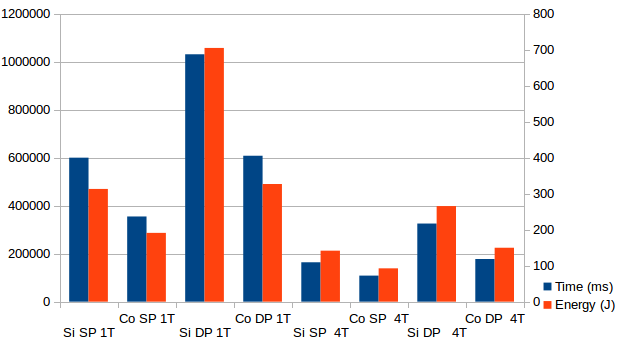
\includegraphics[scale=0.5]{results/A7-1D}
  \caption{Cortex-A7 1-Dimension Stencil}
  \label{pic:A7-1d}
\end{figure}

As with the Cortex-A15 cluster, Table~\ref{tbl:energy-A7-1D} shows that the not-used elements of the CPU (the Cortex-A15 cluster and the GPU) and active elements (the Cortex-A7 cluster and the memory) used energy proportional to the execution time.
\begin{table}[ht]
  \begin{center}
    \begin{tabular}{| l | l | l | l | l | l |}
      \hline
      & Total & A15 & A7 & GPU & Memory \\ \hline
      Si SP 1T & 313.34 & 57.25  & 144.92 & 57.28  & 53.87 \\ \hline
      Co SP 1T & 191.23 & 36.54  & 88.54  & 36.54  & 29.60 \\ \hline
      Si DP 1T & 705.46 & 263.87 & 245.43 & 105.50 & 90.65 \\ \hline
      Co DP 1T & 327.14 & 64.79  & 145.07 & 63.34  & 53.92 \\ \hline
      Si SP 4T & 141.80 & 16.98  & 76.11  & 15.99  & 32.71 \\ \hline
      Co SP 4T & 92.75  & 11.81  & 51.35  & 11.24  & 18.33 \\ \hline
      Si DP 4T & 265.61 & 38.12  & 134.05 & 35.53  & 57.89 \\ \hline
      Co DP 4T & 149.85 & 21.33  & 76.16  & 20.11  & 32.23 \\ \hline
    \end{tabular}
    \caption{1-D Stencil -- Energy  (J) decomposition using the Cortex-A7 cluster}
    \label{tbl:energy-A7-1D}
  \end{center}
\end{table}



\noindent \textbf{2-D Composed Stencil Results} \\
More interesting results come fro the 2-D composed stencil as the computational analysis shows that the computational and memory access cost is worse than in the conventional stencil. But the benchmarks show that although the improvement in both execution time and energy is not as good as in the 1-D case, benefits are significant (except for Hornet using single precision and one thread) specially when using multi-threading and double precision.

\begin{figure}[ht!]
  \centering
  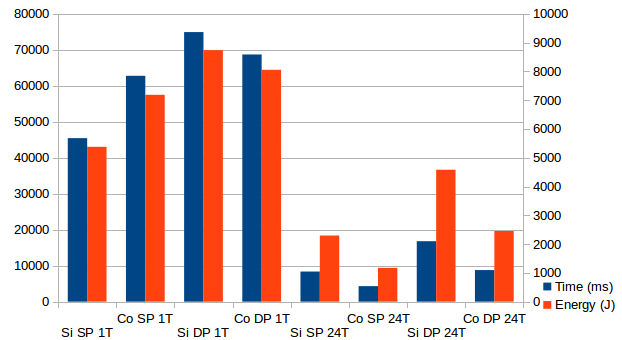
\includegraphics[scale=0.5]{results/Hornet-2D}
  \caption{Hornet 2-Dimension Stencil}
  \label{pic:hornet-2d}
\end{figure}
Figure~\ref{pic:hornet-2d} depicts the results on Hornet. Only in the case were single precision and one thread were used the performance and energy were worse (around 33\%), and all the other cases, both performance and energy used, improved (merely an 8\% for double precision using one thread, and more than a 45\% when multi-threading was used for single and double precision).

Figures~\ref{pic:A15-2d} and \ref{pic:A7-2d} show that for both ARM Cortex types there was a benefit in all cases, but these were less than for Hornet, ranging around 12 to 35\% less execution time and 15 to 25\% reduction in energy used.
\begin{figure}[ht!]
  \centering
  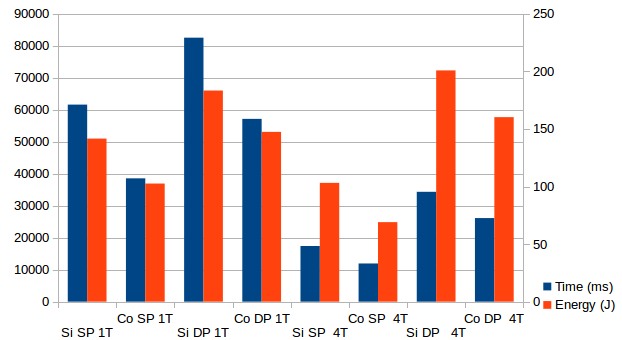
\includegraphics[scale=0.5]{results/A15-2D}
  \caption{Cortex-A15 2-Dimension Stencil}
  \label{pic:A15-2d}
\end{figure}

The energy decomposition for the Cortex-A15 test, Table~\ref{tbl:energy-A15-2D}, shows an increment of the power (energy per unit of time) used by the active cores (5 to 20\%), while the power needed by the memory is reduced (up to a 15\%). The total power needed is bigger but due to the lower running time the total energy used is reduced. For this case the Cortex-A7 test shows very similar results (\textit{c.f.} Table~\ref{tbl:energy-A15-2D}).
\begin{table}[ht]
  \begin{center}
    \begin{tabular}{| l | l | l | l | l | l |}
      \hline
      & Total & A15 & A7 & GPU & Memory \\ \hline
      Si SP 1T & 141.64 & 128.47 & 1.30 & 6.42 & 5.43  \\ \hline
      Co SP 1T & 102.64 & 94.77  & 0.77 & 3.81 & 3.27  \\ \hline
      Si DP 1T & 183.42 & 163.66 & 1.83 & 8.16 & 9.75  \\ \hline
      Co DP 1T & 147.52 & 134.42 & 1.19 & 5.58 & 6.31  \\ \hline
      Si SP 4T & 103.18 & 96.00  & 0.64 & 2.43 & 4.10  \\ \hline
      Co SP 4T & 69.08  & 63.33  & 1.49 & 1.90 & 2.34  \\ \hline
      Si DP 4T & 200.94 & 184.02 & 1.36 & 5.48 & 10.07 \\ \hline
      Co DP 4T & 160.32 & 147.48 & 1.40 & 4.24 & 7.19  \\ \hline
    \end{tabular}
    \caption{2-D Stencil -- Energy (J) decomposition using the Cortex-A15 cluster}
    \label{tbl:energy-A15-2D}
  \end{center}
\end{table}


%Figure~\ref{pic:A7-2d}
\begin{figure}[ht!]
  \centering
  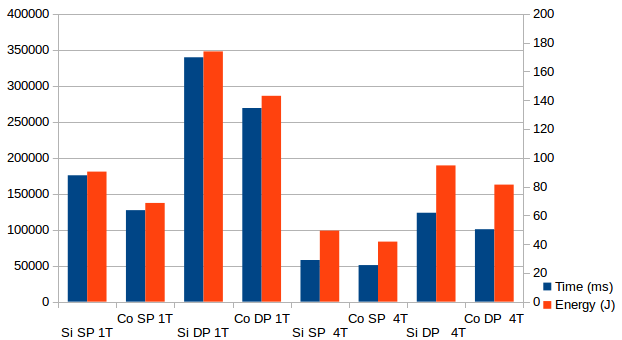
\includegraphics[scale=0.5]{results/A7-2D}
  \caption{Cortex-A7 2-Dimension Stencil}
  \label{pic:A7-2d}
\end{figure}

\begin{table}[ht]
  \begin{center}
    \begin{tabular}{| l | l | l | l | l | l |}
      \hline
      & Total & A15 & A7 & GPU & Memory \\ \hline
      Si SP 1T & 90.38&	 16.73&	43.13&	16.73&	13.77 \\ \hline
      Co SP 1T & 68.61&	 13.71&	32.94&	12.61&	9.33 \\ \hline
      Si DP 1T & 173.95& 35.70&	78.79&	34.69&	24.76 \\ \hline
      Co DP 1T & 143.07& 28.39&	64.69&	28.19&	21.78 \\ \hline
      Si SP 4T & 49.38&	 6.41&	27.16&	5.97&	9.83 \\ \hline
      Co SP 4T & 41.73&	 5.46&	23.26&	5.14&	7.85 \\ \hline
      Si DP 4T & 94.70&	 14.10&	47.72&	12.98&	19.89 \\ \hline
      Co DP 4T & 81.37&	 12.88&	40.16&	10.86&	17.46 \\ \hline
    \end{tabular}
    \caption{2-D Stencil -- Energy (J) decomposition using the Cortex-A7 cluster}
    \label{tbl:energy-A7-2D}
  \end{center}
\end{table}



\noindent \textbf{3-D Composed Stencil Results} \\
The benchmarks performed for the 3-D composed stencil and depicted in Figure~\ref{pic:hornet-3d} show that the performance and energy used by the Hornet node is improved (up to almost 30\% less execution time and 20\% less energy if multi-threading is used) but that both performance and energy may sensible deteriorate in single-threaded scenarios.
\begin{figure}[ht!]
  \centering
  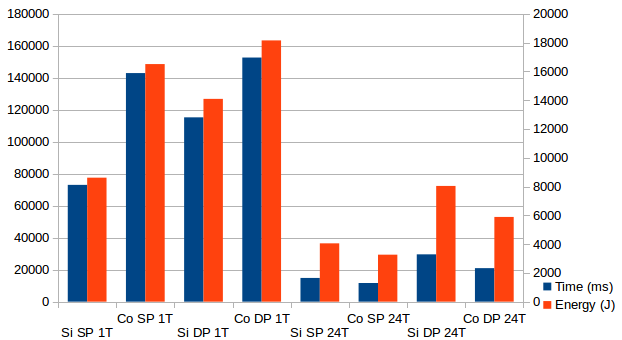
\includegraphics[scale=0.5]{results/Hornet-3D}
  \caption{Hornet 3-Dimension Stencil}
  \label{pic:hornet-3d}
\end{figure}

Similarly, \textit{c.f.} Figure~\ref{pic:A15-3d}, the Cortex-A15 deteriorates its performance and energy consumption in case of composed 3-D stencil in single threaded tests. In multi-threading and single precision the performance is reduced (execution time increases a 32\%) but energy consumption is also reduce almost a 18\%, \textit{i.e.} it takes more time to compute but it uses less energy in total. For the multi-threading and double precision case performance improves a 10\% and energy consumption does not vary (it is reduced less than a 1\%).
\begin{figure}[ht!]
  \centering
  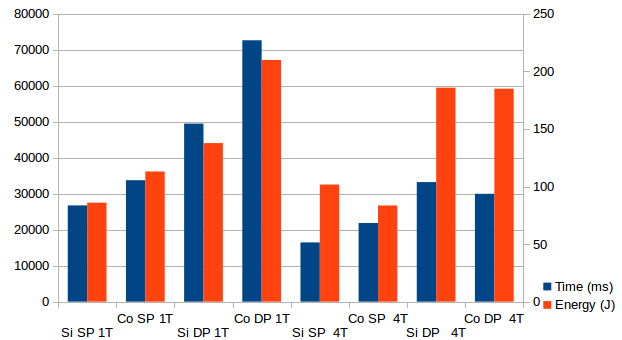
\includegraphics[scale=0.5]{results/A15-3D}
  \caption{Cortex-A15 3-Dimension Stencil}
  \label{pic:A15-3d}
\end{figure}

From Table~\ref{tbl:energy-A15-3D} can be observed that for both single-threaded cases the memory power was less and that the active cores needed more power, having a longer run time the total energy used significantly increased. In the multi-threaded single precision case the power used by the active cores and the memory was greatly reduced and compensated the higher total running time leading to a total energy reduction compared to the single-thread case. In the multi-threaded double precision case the power used by the memory was decreased but the cores needed more power making the system use more power, the total running time was less so the total energy used was slightly less.
\begin{table}[ht]
  \begin{center}
    \begin{tabular}{| l | l | l | l | l | l |}
      \hline
      & Total & A15 & A7 & GPU & Memory \\ \hline
      Si SP 1T & 86.03  & 77.42  & 0.71 & 3.24 & 4.65405 \\ \hline
      Co SP 1T & 113.10 & 103.16 & 0.84 & 3.94 & 5.14199 \\ \hline
      Si DP 1T & 137.75 & 121.42 & 1.15 & 5.21 & 9.9518  \\ \hline
      Co DP 1T & 209.91 & 189.65 & 1.58 & 7.36 & 11.3083 \\ \hline
      Si SP 4T & 101.78 & 93.20  & 0.76 & 2.34 & 5.47308 \\ \hline
      Co SP 4T & 83.60  & 74.51  & 1.41 & 3.16 & 4.51311 \\ \hline
      Si DP 4T & 185.90 & 168.55 & 1.24 & 4.74 & 11.3577 \\ \hline
      Co DP 4T & 185.02 & 170.13 & 1.34 & 4.76 & 8.78189 \\ \hline
    \end{tabular}
    \caption{3-D Stencil -- Energy (J) decomposition using the Cortex-A15 cluster}
    \label{tbl:energy-A15-3D}
  \end{center}
\end{table}


Figure~\ref{pic:A7-3d} clearly shows that for the Cortex-A7 cores the composed 3-D stencil reduces performance and increases energy consumption.
\begin{figure}[ht!]
  \centering
  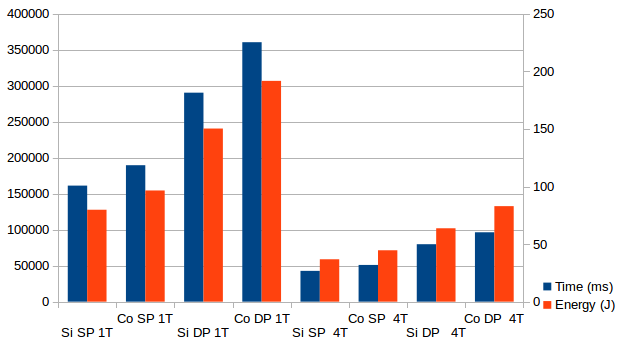
\includegraphics[scale=0.5]{results/A7-3D}
  \caption{Cortex-A7 3-Dimension Stencil}
  \label{pic:A7-3d}
\end{figure}

Table~\ref{tbl:energy-A7-3D} clarifies that even if the power needed by the memory is decreased the active cores increase their power needs, making the system more energy hungry. As the computation time also increases for all the tests, the energy used in every test is also increased.
\begin{table}[ht]
  \begin{center}
    \begin{tabular}{| l | l | l | l | l | l |}
      \hline
               & Total  & A15   & A7    & GPU   & Memory \\ \hline
      Si SP 1T & 79.83  & 14.48 & 37.50 & 14.16 & 13.67  \\ \hline
      Co SP 1T & 96.62  & 17.85 & 46.98 & 18.00 & 13.78  \\ \hline
      Si DP 1T & 150.43 & 30.24 & 67.20 & 29.17 & 23.82  \\ \hline
      Co DP 1T & 191.82 & 37.32 & 89.56 & 37.51 & 27.42  \\ \hline
      Si SP 4T & 36.83  & 5.12  & 19.84 & 4.45  & 7.39   \\ \hline
      Co SP 4T & 44.66  & 5.40  & 27.00 & 5.10  & 7.14   \\ \hline
      Si DP 4T & 63.73  & 8.86  & 32.57 & 8.25  & 14.03  \\ \hline
      Co DP 4T & 82.99  & 10.88 & 46.92 & 10.42 & 14.76  \\ \hline
    \end{tabular}
    \caption{3-D Stencil -- Energy (J) decomposition using the Cortex-A7 cluster}
    \label{tbl:energy-A7-3D}
  \end{center}
\end{table}



%%%%%%%%%%%%%%%%%%%%%%%%%%%%%%%%%%%%%%%%%%%%%%%%%%%%%%%
%%%%%%%%%%%%%%%%%%%%%%%%%%%%%%%%%%%%%%%%%%%%%%%%%%%%%%%

\section{Conclusions}
\label{conclusions}
Stencil kernels are relevant for science, engineering and image processing, and often take a high percentage of the computation in the applications of these fields. In this work we have exposed a way to compose iterative stencils or combine different ones into a single kernel, reducing the total number of iterations over the original data-grid. With this approach we have demonstrated that it is possible to achieve reduction of the execution time and energy used of over a 40\% for 2-dimensional stencils and 30\% for 3-dimensional stencils in HPC machines. For systems with a more limited memory subsystem, such as many ARM-based systems, the improvements for 2-dimensional stencils are also noticeable but might not be for 3-dimensional stencils. The best results were achieved from 1-dimensional stencils, but these have very little applicability in real-life problems. We have also seen that the combination of stencil kernels is a mechanical process, thus it should be possible to automatize it in future.

In will be interesting to analyze how the combination of stencils affects hardware accelerator, in particular FPGAs. We can hypothesize that this approach can benefit them as they can take advantage from the reduced amount of times that the data has to be streamed to them.
 
%
% The following two commands are all you need in the
% initial runs of your .tex file to
% produce the bibliography for the citations in your paper.
\bibliographystyle{abbrv}
\bibliography{paper}


\balancecolumns
\end{document}
